\vspace{-0.3cm}
\section{Evaluation}
\vspace{-0.1cm}
\niparagraph{Image quality.}
%
Figure~\ref{fig:quality} visualizes the output image quality of the FP16 model and \sysname, demonstrating that \sysname's output image quality matches that of FP16. 
%
Table~\ref{tab:quality} reports quantitative results for image quality.
%
% Our method achieves the best FID and IS across most models while maintaining a nearly identical CLIP Score to FP16.
%
As Q-DiT and ViDiT-Q are designed to use high activation bitwidths (e.g., INT8/8 or INT4/8), they suffer from poor image quality when using INT6/6 precision.
%
In contrast, our mixed-precision scheme applies MX9 only to activation outliers while using MX6 for the rest, achieving image quality comparable to FP16.
%
% Consequently, \sysname consistently delivers the best or closely-matching-to-FP16 output qualities.

% Figure 는 FP16 model, Ours 에서의 output quality 를 보여준다. 
% 우리의 output quality 가 FP16 만큼 좋다. 
% Table 은 image quality 에서의 quantitative result 이다. 
% baseline Q-DiT 와 ViDiT-Q 는 INT(8/8) 또는 INT(4/8) 같이 높은 activation bitwidth를 대상으로 quantization 을 한 work인데, 이들은 activation bitwidth 가 6bit 로 적어진 INT(6/6) precision 에서는 나쁜 image quality 를 보여준다. 
% MX6 만 사용한 경우에도 마찬가지로 activation outlier 로 인해 생기는 문제들을 해결하지 못해 image quality 가 나쁘다. 
% 우리의 mixed precision scheme 에서는 activation outlier 들을 MX9 으로 양자화하고, 그 외 대부분의 값들은 MX6 로 성공적으로 양자화함으로써 FP16 과 비슷한 image quality 를 얻을 수 있었다. 
% Ours 는 대부분의 모델에서 가장 좋은 FID 및 IS 를 보여주며, FP16 와 거의 비슷한 CLIP Score 를 보여주고 있다. 

% Figure
\begin{figure}[t]
\centering
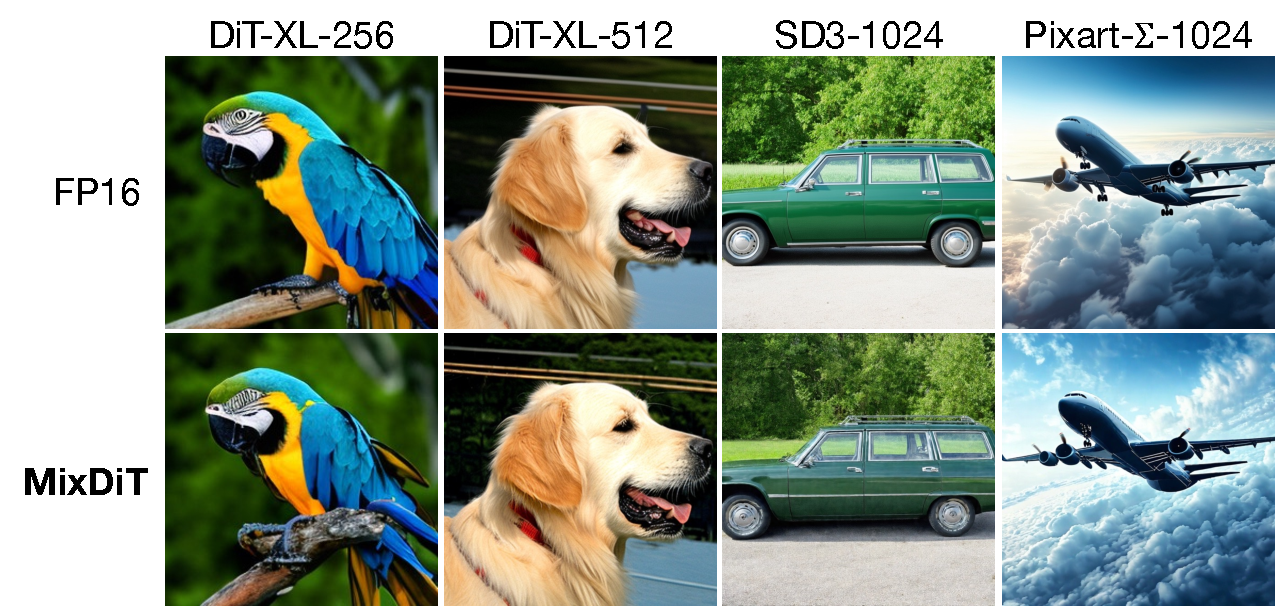
\includegraphics[width=0.8\linewidth]{fig/quality.pdf}
\caption{Images generated by FP16 model and \sysname.}
\label{fig:quality}
\end{figure}

% Table - quality
\begin{table}
\caption{Image quality evaluation}
\label{tab:quality}
\centering
\footnotesize
\begin{tabular}{cccccc} 
\toprule
\begin{tabular}[c]{@{}c@{}}Model\\($p_1$, $p_2$)\end{tabular}                        & \begin{tabular}[c]{@{}c@{}}Precision\\(W/A)\end{tabular} & Method  & FID$\downarrow$   & IS$\uparrow$     & \begin{tabular}[c]{@{}c@{}}CLIP\\score$\uparrow$\end{tabular}  \\ 
\midrule
\multirow{4}{*}{\begin{tabular}[c]{@{}c@{}}DiT-XL-256\\(0, 0)\end{tabular}}    & FP (16/16)      & FP16    & 17.32 & 231.20 &  - \\
    & INT (6/6)       & Q-DiT       & 29.27             & 169.49            &  - \\
    & MX (6/6)        & MX6         & 67.27             & 59.99             &  - \\
    & MX (6/6)        & \sysname    & \textbf{15.39}    & \textbf{232.85}   & - \\ 
\midrule
\multirow{4}{*}{\begin{tabular}[c]{@{}c@{}}DiT-XL-512\\(1, 0)\end{tabular}}    & FP (16/16)      & FP16    & 20.55 & 216.83 & - \\
    & INT (6/6)       & Q-DiT       & \textbf{18.04}    & 209.77            & - \\
    & MX (6/6)        & MX6         & 108.70            & 22.88             & - \\
    & MX (6/6)        & \sysname    & 20.15             & \textbf{217.77}   & - \\ 
\midrule
\multirow{3}{*}{\begin{tabular}[c]{@{}c@{}}SD3-1024\\(5, 20)\end{tabular}}     & FP (16/16)      & FP16    & 74.07    &    -    & \textbf{29.56} \\
    & MX (6/6)        & MX6         & 199.78            &   -    & 22.74 \\
    & MX (6/6)        & \sysname    & \textbf{72.48}    &   -    & 29.34 \\ 
\midrule
\multirow{4}{*}{\begin{tabular}[c]{@{}c@{}}Pixart-$\Sigma$-1024\\(1, 20)\end{tabular}} & FP (16/16)      & FP16    & 69.96    &   -    & 31.34  \\
    & INT (6/6)       & ViDiT-Q     & 84.74             &   -    & \textbf{31.93} \\
    & MX (6/6)        & MX6         & 71.66             &   -    & 31.31          \\
    & MX (6/6)        & \sysname    & \textbf{69.29}    &   -    & 31.50            \\
\bottomrule
\end{tabular}
\end{table}


\niparagraph{Speedup.}
Figure~\ref{fig:speedup} reports \sysname latency speedup compared to the baseline schemes on NVIDIA RTX 3090.
%
% We match our baseline accelerator's TOPS to that of the RTX 3090 when using MX9, making the performance difference between the two platforms negligible.
When using MX9, our baseline accelerator achieves the same TOPS as the RTX 3090 with INT8.
%
% However, leveraging the mixed-precision of MX6 and MX9, \sysname achieves 1.45$\times$ to 2.47$\times$ speedup compared to the GPU. 
Leveraging the mixed-precision of MX6 and MX9, \sysname achieves 2.10$\times$ to 5.32$\times$ speedup compared to the GPU. 
%
We observe that only $\leq$5\% of activations in linear layers and $\leq$20\% of activations in attention layers are quantized with MX9, allowing \sysname to achieve similar speedups to MX6 while minimizing quality loss.
%
% GEMM in the systolic array, channel-wise reordering, and MX conversion were pipelined in hardware.
Quantizing most data to MX6 leverages the 4-bit multipliers, which accelerate systolic array computations and serve as the main contributor to the speedup.
%
We notice that larger image generation models see greater improvement, as GEMM computations dominate latency.
% figure 
\begin{figure}[t]
\centering
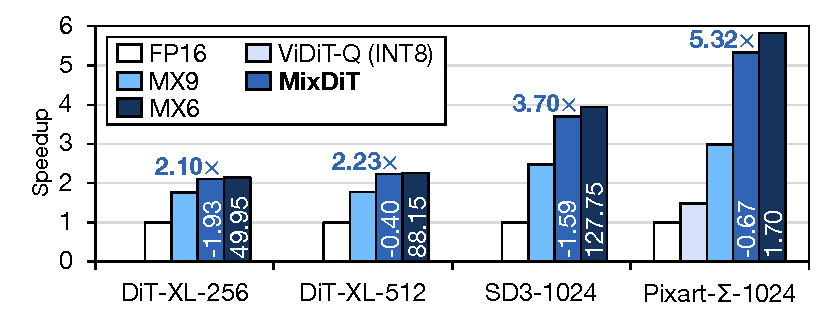
\includegraphics[width=\linewidth]{fig/speedup.pdf}
\caption{Latency speedup compared to RTX 3090. The y-axis represents speedup (higher is better), while the numbers inside the bars indicate FID degradation compared to FP16 (lower is better).}
\label{fig:speedup}
\end{figure}
